\documentclass[11pt,a4paper]{article}

\usepackage[a4paper,left=24mm,right=24mm,top=22mm,bottom=22mm]{geometry}
\usepackage{amsmath,amssymb}
\usepackage{booktabs}
\usepackage{graphicx}
\usepackage[expansion=false]{microtype}
\usepackage{siunitx}
\usepackage{caption}
\usepackage[hidelinks]{hyperref}
\usepackage{enumitem}
\usepackage{xcolor}
\usepackage{tikz}
\usepackage{titlesec}
\usepackage{fancyhdr}

\sisetup{detect-weight=true,detect-family=true,group-separator={,},
         group-digits=integer,group-minimum-digits=4}

\definecolor{accent}{HTML}{2F5D7C}
\definecolor{warm}{HTML}{B5553F}
\definecolor{green2}{HTML}{2F6D4F}
\definecolor{slate}{HTML}{4A5568}
\definecolor{lightbg}{HTML}{EEF2F5}

\titleformat{\section}{\large\bfseries\color{accent}}{\thesection}{0.6em}{}
\titleformat{\subsection}{\normalsize\bfseries}{\thesubsection}{0.6em}{}
\titlespacing*{\section}{0pt}{14pt}{5pt}
\titlespacing*{\subsection}{0pt}{10pt}{3pt}

\captionsetup{font=small,labelfont=bf}
\setlist{itemsep=2.5pt,parsep=0pt,topsep=4pt}

\pagestyle{fancy}\fancyhf{}
\fancyhead[L]{\small\color{slate} Thesis B progress update --- J.\ Mohindra}
\fancyhead[R]{\small\color{slate}\thepage}
\renewcommand{\headrulewidth}{0.4pt}

\newenvironment{keybox}{%
  \par\vspace{5pt}\noindent
  
\begin{tikzpicture}\node[draw=accent,line width=0.8pt,fill=lightbg,rounded corners=2pt,
    inner sep=9pt,text width=\dimexpr\textwidth-24pt\relax,align=justify]\bgroup\small}
  {\egroup;\end{tikzpicture}\par\vspace{5pt}}

\begin{document}

\begin{center}
{\LARGE\bfseries Thesis B --- Progress Update\par}
\vspace{5pt}
{\large Comparison and Implementation of Data Compression Methods\\
for SoC-based Radar Systems\par}
\vspace{10pt}
{\normalsize
Jordan Mohindra (z5418455) \quad$\cdot$\quad
Supervisor: A/Prof.\ Beena Ahmed\quad$\cdot$\quad
17 September 2026\par}
\end{center}
\vspace{4pt}
\hrule
\vspace{10pt}

% ===================================================================
\section*{The short version}

Since the Thesis A report I have built, verified and characterised complete
hardware implementations of \textbf{two} lossless radar compression algorithms
--- DRHE and LPC --- on the Kintex UltraScale+ FPGA, each with a matching
decompressor. Both reconstruct real radar data perfectly: zero error across
\num{157} million samples, confirmed three separate ways.

Then I audited the results, and found something I was not expecting.

\begin{keybox}
\textbf{The main finding.} Applied the way the literature describes them,
\emph{neither predictor was doing anything useful}. Running the same data
through the same entropy coder with \emph{no prediction at all} compressed
\textbf{better} than either algorithm --- \num{3.489} against \num{3.319}
(DRHE) and \num{3.397} (LPC). Both predictors were making the data measurably
harder to compress.

The cause is that our radar is a 12-transmitter TDM-MIMO cascade, and the
transmitters are interleaved along the axis the algorithms predict along. ``The
previous ramp'' is a different physical antenna eleven times out of twelve.
Predicting from the previous ramp of the \emph{same} transmitter fixes it, and
lifts measured compression from \num{3.310} to \num{3.751} for DRHE and
\num{3.385} to \num{3.697} for LPC --- still perfectly lossless. For DRHE the
fix costs \num{40} extra block RAMs (\SI{4}{\percent} of the chip) and
\emph{nothing else}: same logic, same clock speed, same latency.
\end{keybox}

\noindent
I have implemented, verified and synthesised the corrected versions of both
algorithms. I also found and fixed two implementation bugs that would have
shipped, and corrected three factual errors --- one in the literature, two in
my own Thesis A report.

\begin{figure}[h]
\centering
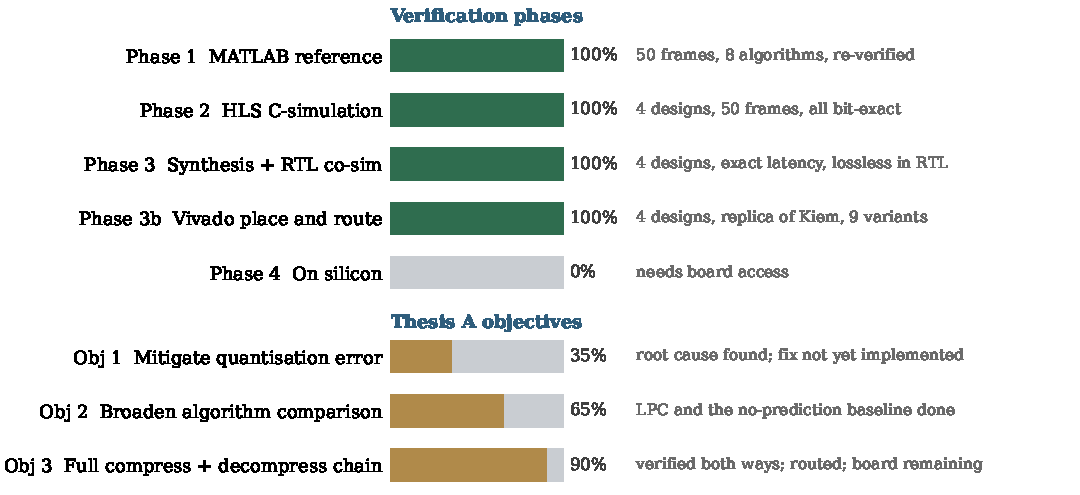
\includegraphics[width=\textwidth]{fig_status.pdf}
\caption{Where the project stands. Phases 1--3 are complete for all four
designs; Phase 4 needs the physical board.}
\end{figure}

% ===================================================================
\section{What I built}

\subsection{The two compressors, in plain terms}

Both algorithms work the same way in outline. They \emph{predict} what the next
radar sample will be from samples already sent, then transmit only the
\emph{difference} between the prediction and reality. When the prediction is
good the differences are tiny, and tiny numbers can be written in very few
bits. Nothing is thrown away --- the receiver runs the same prediction and adds
the difference back --- so the process is exactly lossless.

They differ in how they predict:

\begin{itemize}
\item \textbf{DRHE} converts each sample to magnitude and phase and predicts
each with a fixed filter. It assumes a target's brightness stays roughly
constant and its phase advances by a constant step, which is what a target
moving at constant speed does. It is \emph{streaming}: it needs no buffer and
starts producing output immediately.

\item \textbf{LPC} fits a mathematical model to the data instead of assuming
one. It is more flexible, but it has to see the whole frame before it can fit
the model --- so it needs a \SI{3.1}{\mebi bit} buffer and cannot output
anything until the frame is complete.
\end{itemize}

Both then feed their differences into the same entropy coder, which assigns
short bit patterns to common values and long ones to rare values.

\subsection{Deliverables}

\begin{itemize}
\item DRHE compressor and decompressor in Vitis HLS (C++), synthesised for
\texttt{xcku5p}.
\item LPC compressor and decompressor, likewise.
\item TDM-corrected versions of both, kept alongside the originals so every
comparison is like-for-like.
\item A 50-frame testbench driven by real ColoRadar data exported from MATLAB.
\item An 8-case synthetic edge-case testbench.
\item Four MATLAB audit scripts that produced the findings in
Section~\ref{sec:finding}.
\item A 70-page written report covering all of the above.
\end{itemize}

% ===================================================================
\section{How I verified it}

The single most important property of these compressors is that they are
\emph{exactly} lossless --- a radar that silently loses a weak target to save
bandwidth is not safe. So the verification had to be able to \emph{prove}
exactness, not estimate it. I used a four-stage ladder, each stage checking the
one above it at a lower level:

\begin{enumerate}
\item \textbf{MATLAB, double precision.} The golden reference. Tells us exactly
what bits should come out.
\item \textbf{HLS C-simulation.} The hardware C++ compiled and run as ordinary
software. Asks: does it reproduce MATLAB \emph{bit for bit}?
\item \textbf{RTL co-simulation.} The synthesised hardware, simulated
cycle-by-cycle. Asks: did synthesis change anything? Also gives exact latency.
\item \textbf{On silicon.} Not yet done --- needs the board.
\end{enumerate}

\noindent
Every design passes stages 1--3 with \textbf{zero} reconstruction error over
all 50 frames.

Agreement with MATLAB is tighter than I set as the pass criterion. For LPC, a
MATLAB model that accounts for AXI packet padding reproduces the hardware bit
count on \num{50} of \num{50} frames to within $5\times10^{-6}$ --- meaning the
underlying bit counts are identical and the only difference is packet padding.

% ===================================================================
\section{Results before the audit}

\subsection{MATLAB benchmark (all 8 algorithms, 50 frames, 16 RX)}

\begin{table}[h]
\centering
\small
\caption{Detection metrics are against a double-precision reference.
\emph{FN} is missed detections; \emph{FDR} is what fraction of reported
detections were spurious.}
\begin{tabular}{@{}lrrrl@{}}
\toprule
Algorithm & CR & FN\% & FDR\% & \\
\midrule
FP16          & 1.00 & 0.00  & 0.00 & reference-quality, no compression\\
FX16          & 1.00 & 3.77  & 1.11 & the quantisation step alone\\
\textbf{DRHE} & \textbf{3.30} & 3.77 & 1.11 & lossless\\
\textbf{LPC}  & \textbf{3.37} & 3.77 & 1.11 & lossless\\
BAQ           & 3.76 & 10.44 & 9.69 & lossy --- note the detection cost\\
RDVLE         & 1.12 & 24.01 & 4.62 & lossy\\
RDVLE\_UDRE   & 2.56 & 28.73 & 4.44 & lossy\\
\bottomrule
\end{tabular}
\end{table}

Two points worth making to anyone reading this table:

\begin{itemize}
\item \textbf{DRHE, LPC and FX16 have identical detection metrics by
construction}, not by coincidence. All three reconstruct the quantised data
perfectly, so the detector sees identical input. What those rows actually
measure is the cost of the \emph{quantisation} step, not of compression.

\item \textbf{BAQ shows why lossless matters.} It reaches a slightly better
ratio but misses nearly three times as many real targets and invents nearly
nine times as many false ones. That is not a trade worth taking in a braking
system.
\end{itemize}

\subsection{Hardware (synthesis, \texttt{xcku5p} at \SI{100}{\mega\hertz})}

\begin{table}[h]
\centering
\small
\begin{tabular}{@{}lrrr@{}}
\toprule
& DRHE & LPC & Kiem's design \\
\midrule
LUT           & \num{115534} & \num{80528} & \num{45892}\\
Flip-flops    & \num{57105}  & \num{17393} & \num{9243}\\
Block RAM (18\,Kb) & \num{40}     & \num{256}   & \num{20}$^{*}$\\
DSP slices    & \num{132}    & \num{168}   & \num{44}\\
Max clock     & \SI{81.9}{\mega\hertz} & \SI{85.4}{\mega\hertz} & \SI{100}{\mega\hertz}\\
Frame latency & \num{61253} cycles & \num{197277} cycles & ---\\
Frame buffer  & none & \SI{3.1}{\mebi bit} & ---\\
\bottomrule
\end{tabular}

\smallskip
{\footnotesize $^{*}$Kiem reports 10 in 36\,Kb tiles. Our figures are HLS
estimates; his are post-implementation.}
\end{table}

\noindent
\textbf{How to read these numbers.} On their own they say little; each needs a
yardstick, and the report now has a chapter giving one for every metric. The
short version: DRHE accepts data \num{24.6} times faster than four ColoRadar
channels produce it, uses \num{319} of the \num{7850} cycles available per
ramp, and adds only \SI{3.2}{\micro\second} after the last ramp of a frame
(LPC adds \SI{3}{\milli\second}). So it passes every \emph{performance}
requirement by a wide margin. Where it falls short is \emph{cost}: 2.5 times
Kiem's LUTs, which would not fit his ZU3EG at all (\SI{164}{\percent}), and
\SI{81.9}{\mega\hertz} against a \SI{100}{\mega\hertz} system clock. Both
shortfalls come from the floating-point datapath.

\noindent
The surprise here was that \textbf{LPC is the cheaper design}, not the more
expensive one. I had expected its division to dominate. It does not --- the
division runs \num{1024} times per frame and accounts for \SI{0.26}{\percent}
of the cycles. What actually costs is DRHE's four floating-point
transcendental functions (\texttt{sqrt}, \texttt{atan2}, \texttt{sin},
\texttt{cos}) evaluated for every sample of every channel. The real trade is
\textbf{logic (DRHE) against memory and latency (LPC)}.

Neither design closes timing at \SI{100}{\mega\hertz}. Both fixes are
identified (Section~\ref{sec:next}).

% ===================================================================
\section{The main finding: we were predicting along the wrong axis}
\label{sec:finding}

\subsection{How I found it}

At this point every test passed and the compression ratios matched the
literature, so the obvious conclusion was that the work was done. Before
writing it up I ran one extra check that is not part of any standard
compression evaluation:

\begin{center}
\emph{What happens if I remove the predictor entirely and code the raw data
through the same entropy coder?}
\end{center}

\noindent
Anything that survives is the entropy coder's doing, not the predictor's.

\begin{table}[h]
\centering
\small
\begin{tabular}{@{}lrrr@{}}
\toprule
Configuration & bits/value & CR & vs.\ no prediction\\
\midrule
\textbf{No prediction at all} & \textbf{4.586} & \textbf{3.489} & --- \\
DRHE as implemented           & 4.821 & 3.319 & $0.951\times$ \emph{(worse)}\\
LPC as implemented            & 4.710 & 3.397 & $0.974\times$ \emph{(worse)}\\
\bottomrule
\end{tabular}
\end{table}

\noindent
Both predictors were \emph{costing} bits. An independent check confirms it:
the information content (order-0 entropy) of the raw data is
\SI{4.094}{bits}, and of the DRHE differences \SI{4.538}{bits}. The predictor
was \emph{increasing} the entropy of data it was supposed to be simplifying.

\subsection{Why}

Our radar has 12 transmit antennas that fire one at a time in rotation. When
the data is laid out for a streaming compressor, the ``ramp'' index is
\[
m = (\text{chirp loop}) \times 12 + (\text{transmitter index}),
\]
so the transmitter changes \emph{every single ramp}. Ramp $m$ and ramp $m-1$
were transmitted by different antennas, in different physical positions. The
difference between them is dominated by \emph{where the target is in angle},
not by how fast it is moving --- and it jumps around on a period-12 pattern
that neither algorithm can track.

The genuine slow-time neighbour --- the one whose difference reflects target
\emph{motion} --- is ramp $m-12$.

\begin{keybox}
This is not a bug in Kiem's work. On a single-transmitter radar, which is what
his specification addresses, ramp $m-1$ \emph{is} the correct neighbour. The
error is in applying that specification unmodified to a MIMO sensor of a
different kind --- which is what I did before measuring it.
\end{keybox}

\subsection{What it looks like on real data}

Figure~\ref{fig:worked} shows sixteen consecutive ramps of one range bin, run
through the same DRHE predictor twice. Only the prediction lag differs.

\begin{figure}[h]
\centering
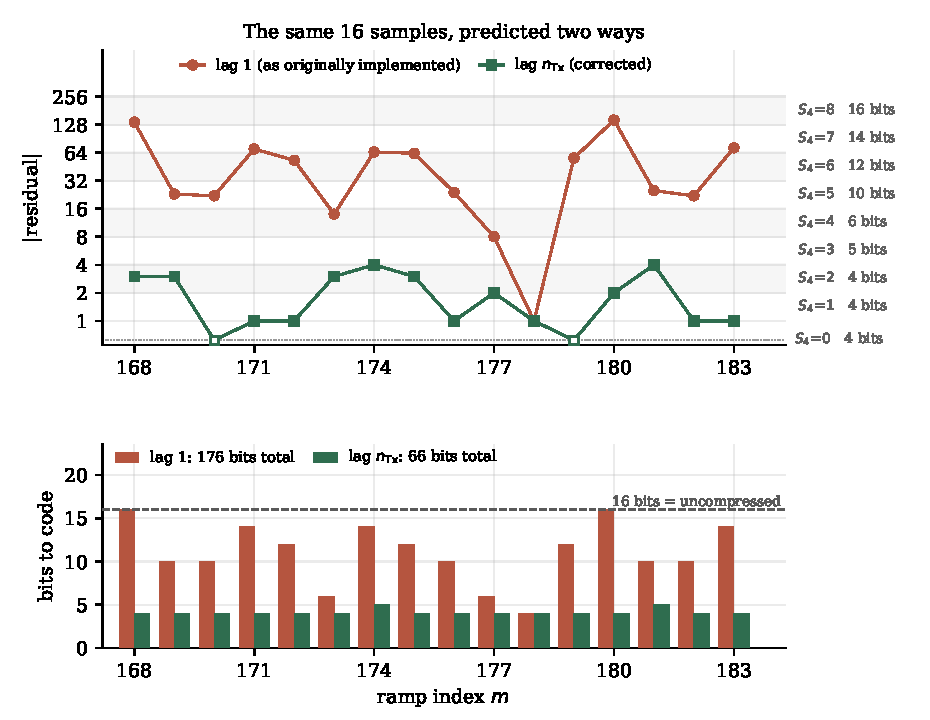
\includegraphics[width=0.92\textwidth]{fig_worked.pdf}
\caption{The same sixteen real samples, predicted two ways. Above: the size of
each difference, with the bit-cost bands of the entropy coder marked. Below:
what each sample costs. Predicting from the previous ramp spends \num{176}
bits; predicting from the previous ramp of the same transmitter spends
\num{66} --- for identical information.}
\label{fig:worked}
\end{figure}

The underlying reason is visible in the raw numbers. Against ramp $m-1$, the
target's phase step swings over $\pm 2.6$ radians with no pattern. Against ramp
$m-12$, it is $0.002$, $-0.040$, $0.017$, $-0.008$ --- essentially zero,
because it is a stationary target and twelve ramps later the same antenna sees
the same thing.

\subsection{The fix, and what it costs}

\begin{table}[h]
\centering
\small
\caption{Corrected designs against their originals. Vitis HLS C-simulation,
all 50 frames. Everything remains exactly lossless.}
\begin{tabular}{@{}lrrrrrr@{}}
\toprule
Design & CR & MaxDiff & LUT & FF & BRAM & Latency (cyc)\\
\midrule
DRHE, original      & \num{3.30987} & 0 & \num{115534} & \num{57105} & \num{40} & \num{61253}\\
\textbf{DRHE, corrected} & \textbf{\num{3.75082}} & \textbf{0} & \num{115736} & \num{57263} & \num{80} & \num{61253}\\
\addlinespace
LPC, original       & \num{3.38497} & 0 & \num{80528} & \num{17393} & \num{256} & \num{197277}\\
\textbf{LPC, corrected}  & \textbf{\num{3.69681}} & \textbf{0} & \num{86298} & \num{23154} & \num{192} & \num{325166}\\
\bottomrule
\end{tabular}
\end{table}

\begin{itemize}
\item \textbf{DRHE: \SI{+13.3}{\percent} compression for 40 block RAMs.}
Logic, DSPs, clock speed and measured frame latency are all unchanged. The
extra memory holds one copy of the predictor's state per transmitter. This is
about as close to a free improvement as hardware gets.

\item \textbf{LPC: \SI{+9.2}{\percent}, and a genuine trade.} Restructuring
for the deeper lags happened to fix an unrelated bottleneck --- block RAM drops
\SI{25}{\percent} and every loop now runs at full rate, which the original
never achieved. But the frame takes \num{1.65}$\times$ longer. I have
identified how to recover most of that.
\end{itemize}

Figure~\ref{fig:perframe} shows the improvement is uniform, not an average
artefact --- the corrected designs beat their originals on every single frame.

\begin{figure}[h]
\centering
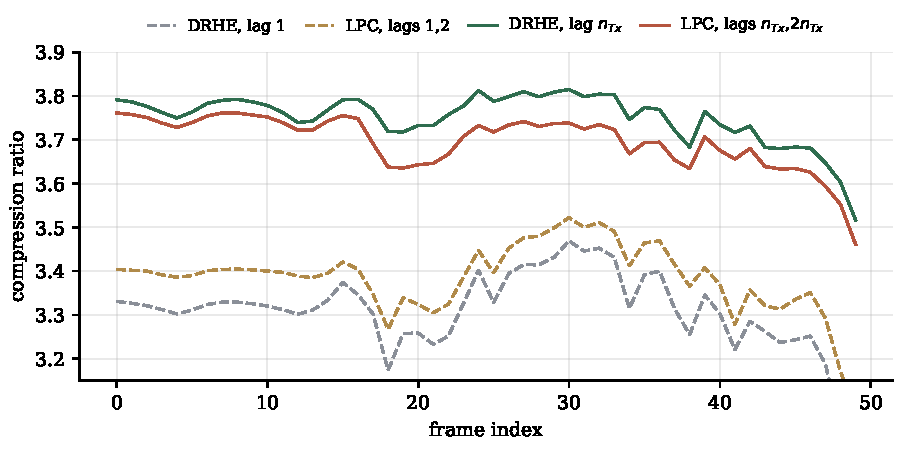
\includegraphics[width=0.88\textwidth]{fig_perframe.pdf}
\caption{Per-frame compression ratio across the 50-frame sequence.}
\label{fig:perframe}
\end{figure}

% ===================================================================
\section{Second finding: what a compression ratio actually measures}

The same audit answered a question I had not thought to ask: \emph{where does
the \num{3.5} come from, if not from prediction?}

\begin{figure}[h]
\centering
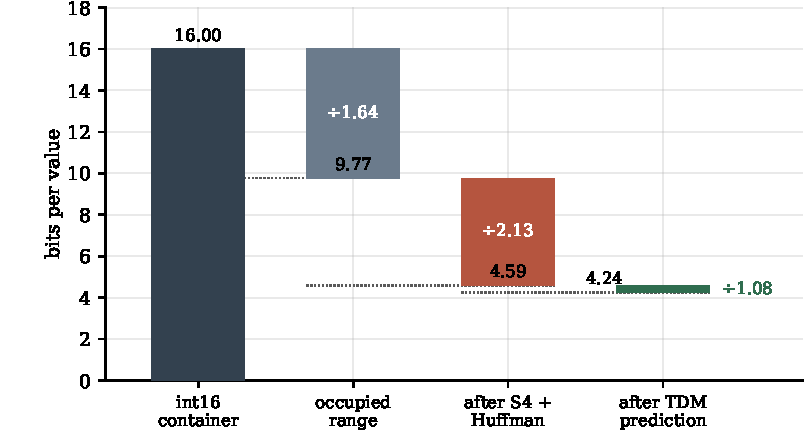
\includegraphics[width=0.62\textwidth]{fig_waterfall.pdf}
\caption{The compression ratio decomposed.}
\end{figure}

\begin{itemize}
\item \textbf{A factor of \num{1.63} is unused container headroom.} Our
quantisation step scales the data assuming a full-scale ADC input. The
ColoRadar recording sits far below that --- its peak raw sample is \num{914}
out of a possible \num{32767}, and after processing the peak 16-bit code is
\num{436}. \textbf{Only \num{9.8} of the \num{16} bits ever carry
information}; the other \num{6.2} are zero in every sample. Any entropy coder
removes them for free.

\item \textbf{A factor of \num{2.14} is genuine.} Radar range-FFT data is
sparse --- most bins are noise near zero --- and that is real, transferable
compression.

\item \textbf{The rest is prediction}, which as implemented was negative and
after the correction is about \num{1.08}.
\end{itemize}

\begin{keybox}
\textbf{Why this matters beyond our project.} It means the compression ratios
reported in this field --- ours and others' --- are substantially a property of
the \emph{sensor's gain setting} rather than of the algorithm. A better-scaled
recording would compress measurably less on identical code. I think reporting a
no-prediction baseline alongside any such figure should be standard, and as far
as I can find, it is not.

It also points directly at Thesis A Objective 1. We are currently wasting
\num{6.2} bits of dynamic range at exactly the point where weak targets are
being crushed into the quantisation noise.
\end{keybox}

% ===================================================================
\section{Two bugs found and fixed}

Both were invisible on real data and both were caught by the synthetic
edge-case suite. Both would have shipped.

\subsection{An unrepresentable value}

The entropy coder's largest category holds exactly $2^{15}$ values, which
exactly fills its payload field --- leaving no room for the value $-32768$,
which 16-bit arithmetic can produce. Encoding it produces bit-for-bit the same
output as $+32767$, and the decoder returns the wrong number. The edge-case
test showed a reconstruction error of \num{65535}, which is precisely the
distance between those two values.

The fix is to clamp $-32768$ to $-32767$ --- but clamping alone is not enough.
Once the reconstruction differs from the original by even one bit, the encoder
and decoder start predicting from different histories and \emph{diverge}, with
the error growing through every remaining ramp. The complete fix is to have the
encoder reconstruct exactly what the decoder will see and predict from
\emph{that}. This costs pipeline depth but bounds the error to one sample.

\subsection{A silent numerical failure}

LPC's solver needs products of large integers, computed as 128-bit values.
Converting one of those directly to floating point is incorrect above $2^{64}$
in this toolchain --- it returns zero. A determinant of $4.4\times10^{20}$ was
converting to $-1.2\times10^{18}$, the wrong sign. Fixed by scaling all the
operands down by a common shift before dividing, which leaves the answer
unchanged.

On real data the numbers involved only reach 44 bits, so this was entirely
unreachable with our dataset.

\begin{keybox}
\textbf{Methodological point worth recording.} Fifty frames of real data ---
\num{157} million samples --- found neither bug. An eight-case synthetic suite
found both in minutes. Conversely, the synthetic suite would never have found
the prediction-axis error, because synthetic data has no transmitter structure
to get wrong. The two kinds of testing find different classes of problem and
neither substitutes for the other.
\end{keybox}

% ===================================================================
\section{Corrections to the record}

Three factual errors surfaced during the audit. I mention them because two are
mine and should be fixed before submission.

\begin{enumerate}
\item \textbf{A throughput figure in the literature is in the wrong units.}
Kiem reports \SI{11.92}{Gbit\per\second}. Read as decimal that is \num{119.2}
bits per clock cycle on a 128-bit bus --- an odd number. Read as
\emph{gibibits} it is \num{127.99}, i.e.\ exactly \num{128} --- the full bus
width at one sample per cycle. The figure is binary; its decimal equivalent is
\SI{12.80}{Gbit\per\second}. Every comparison against \num{11.92} understates
the gap by \SI{7.4}{\percent}. It is also a \emph{theoretical} figure (bus
width $\times$ clock), not a measurement, so it should be compared with our
theoretical \SI{6.4}{Gbit\per\second} (a factor of 2, from II) rather than our
measured \SI{5.14}{}. Likewise his 10 BRAM are 36\,Kb tiles, i.e.\ 20 in our
units: our baseline uses 2 times as much, not 4 times.

\item \textbf{Our ``false positive rate'' is a false discovery rate.} It
divides by the number of \emph{reported} detections, not by the number of true
negatives. It is a legitimate metric --- arguably the more useful one here ---
but it is not what the name denotes.

\item \textbf{Two citations in the Thesis A executive summary are wrong.} The
BAQ reference should be Kwok \& Johnson, IEEE TGRS vol.~27 no.~4 pp.~375--383
(1989), on \emph{synthetic} aperture radar; the name and page range currently
cited do not correspond to any such paper. The ColoRadar reference should be
IJRR vol.~41 no.~4 pp.~351--360 (2022), not vol.~40 (2021). Also, ``simulated
aperture radar'' should read ``synthetic'' throughout.
\end{enumerate}

\noindent
Separately: the DRHE description in Thesis A \S2.5.3 does not match what is
actually implemented. It describes differencing \emph{raw ADC} samples and
coding with Golomb--Rice. The real algorithm operates on the \emph{range-FFT
output}, predicts in polar coordinates with two IIR filters, and codes with a
fixed Huffman dictionary. Worth reconciling before submission.

% ===================================================================
\section{Progress against the Thesis A objectives}

\begin{center}
\small
\begin{tabular}{@{}p{45mm}p{12mm}p{75mm}@{}}
\toprule
Objective & Status & Notes\\
\midrule
\textbf{1. Mitigate quantisation error} & \SI{35}{\percent} &
Root cause now precisely characterised: only \num{9.8} of \num{16} bits are in
use. An adaptive per-frame scale factor is a simpler and larger win than either
approach proposed in Thesis A. Not yet implemented.\\
\addlinespace
\textbf{2. Broaden the algorithm comparison} & \SI{65}{\percent} &
LPC fully implemented and characterised in hardware; BAQ and RDVLE benchmarked
in MATLAB; a no-prediction baseline added, which turned out to be the most
informative comparison of all. NXP CP4/CP8 and AdaRadar not attempted.\\
\addlinespace
\textbf{3. End-to-end hardware} & \SI{85}{\percent} &
Compression \emph{and} decompression implemented for both algorithms and
verified bit-exactly through RTL co-simulation. Remaining: place-and-route,
and running it on the physical board.\\
\bottomrule
\end{tabular}
\end{center}

% ===================================================================
\section{Next steps}
\label{sec:next}

In the order I propose tackling them.

\subsection{High value, low effort}

\begin{enumerate}
\item \textbf{Adaptive FX16 scale factor.} Directly addresses Objective 1,
recovers roughly 6 bits of dynamic range where weak targets currently die, and
makes our reported compression ratios reflect the algorithm rather than the
recording. Probably the single highest-value change remaining.

\item \textbf{Fix DRHE's initiation interval.} The design currently accepts one
sample every \emph{two} cycles instead of every cycle, because of a memory port
conflict caused by a reset that runs on one ramp in \num{192}. Hoisting that
reset out of the loop should roughly double throughput, to
\SI{11}{}--\SI{12}{Gbit\per\second} --- close to Kiem's theoretical
\SI{12.8}{}. This is not needed to keep up with the sensor, which the current
design already does 24.6 times over; it matters for serving all 16 channels
from one instance, or for larger sensors.

\item \textbf{Recover LPC's latency.} The corrected LPC makes two short passes
where it used to make one long one, and pays a pipeline start-up cost
\num{512} times over. Merging the passes should recover most of the
\num{65000} lost cycles.
\end{enumerate}

\subsection{Medium effort}

\begin{enumerate}[resume]
\item \textbf{Replace the polar conversion with a fixed-point CORDIC.} The four
floating-point transcendentals dominate DRHE's logic usage \emph{and} its
critical path, so this addresses both the resource count and the
\SI{81.9}{\mega\hertz} clock ceiling in one change.

\item \textbf{Re-derive the Huffman dictionary.} After the correction,
\SI{86}{\percent} of differences fall into the three cheapest categories, which
is a more concentrated distribution than the current fixed dictionary assumes.
A dictionary matched to the corrected data is a cheap few per cent.

\item \textbf{Place-and-route, then Phase 4 on the board.} Real $F_{\max}$,
real resource counts, power measurement, end-to-end latency.
\end{enumerate}

\subsection{If time allows}

\begin{enumerate}[resume]
\item Benchmark against NXP CP4/CP8 and AdaRadar, completing Objective 2.
\item Check whether the prediction-axis issue has an analogue in
Doppler-division or code-division MIMO, which distribute the slow-time
structure differently.
\end{enumerate}

% ===================================================================
\section{Risks and open questions}

\begin{itemize}
\item \textbf{Board access is the critical path for Phase 4.} Everything else
can proceed in simulation, but power and real timing cannot.

\item \textbf{Timing closure.} Neither design meets \SI{100}{\mega\hertz}
today. The CORDIC change should fix it; if it does not, the fallback is to
report an \SI{80}{\mega\hertz} clock honestly, which still leaves useful
throughput.

\item \textbf{All hardware numbers are pre-implementation estimates.}
Post-route $F_{\max}$ is typically lower than the synthesis estimate.

\item \textbf{Scope.} Objective 2 is only partly done. I would rather finish
the quantisation work (Objective 1) properly than add two more algorithms to
the comparison --- but that is a judgement call worth discussing.
\end{itemize}

\subsection*{Things I would like your view on}

\begin{enumerate}
\item \textbf{Is the prediction-axis finding worth writing up separately?} As
far as I can establish it is not reported anywhere, it applies to any
slow-time predictive coder on a TDM-MIMO radar, and the check that exposes it
costs about twenty lines of MATLAB.

\item \textbf{Should I prioritise the adaptive quantisation work over widening
the algorithm comparison?} My instinct is yes --- it is the original Objective 1,
it is now a well-characterised problem rather than a vague one, and it would
improve the data every algorithm sees.

\item \textbf{What is the realistic timeline for board access?}

\item \textbf{How should the Thesis A corrections be handled} --- a corrigendum,
or simply fixed in the Thesis B document?
\end{enumerate}

% ===================================================================
\section*{Where everything lives}

\begin{table}[h]
\centering
\small
\begin{tabular}{@{}ll@{}}
\toprule
\texttt{ThesisA/Matlab\_Sim/} & MATLAB pipeline, benchmarks and audit scripts\\
\texttt{ThesisA/hls\_component/} & all four HLS designs, testbenches, build configs\\
\texttt{ThesisA/paper/} & the 70-page written report and its figures\\
\texttt{ThesisA/drhe\_testing\_plan.md} & full test plan with every result recorded inline\\
\bottomrule
\end{tabular}
\end{table}

\noindent
Everything is committed to git, with the audit and the correction in their own
commits so the before/after comparison is reproducible.

\end{document}
